\chapter{Senozon Via}
\label{ch:via}
% ##################################################################################################################

\hfill \textbf{Author:} Marcel Rieser

\begin{center} 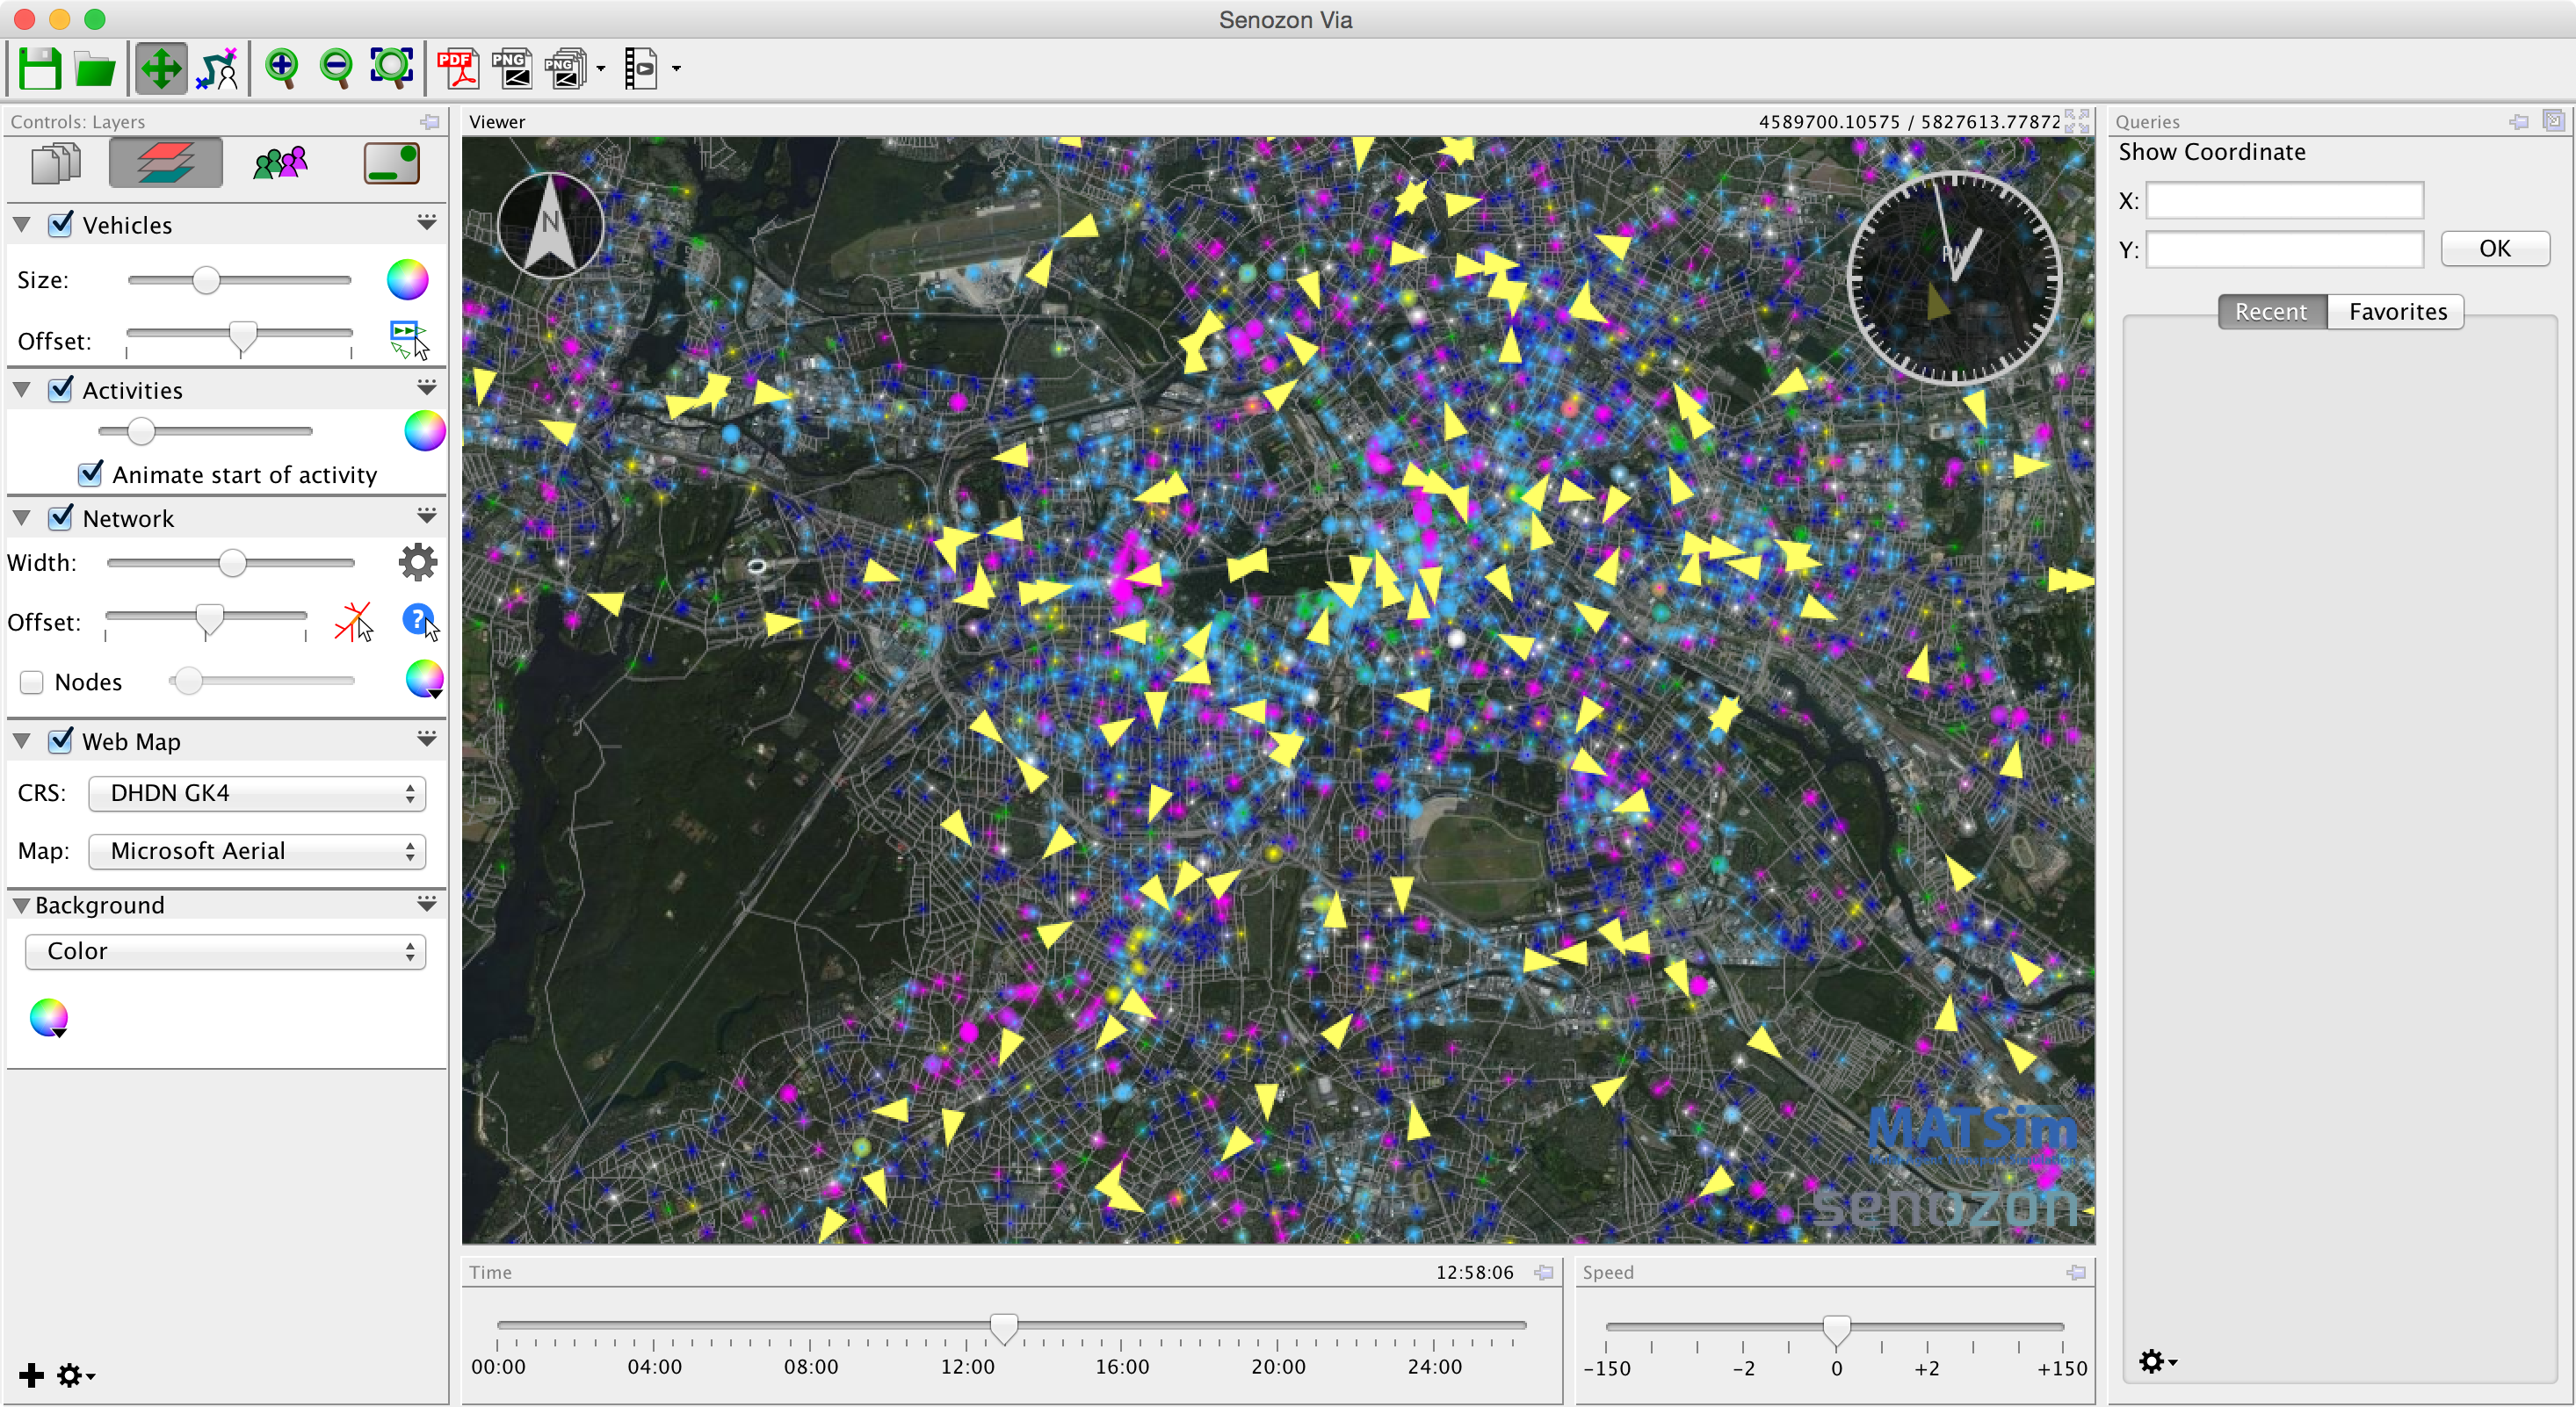
\includegraphics[width=1.\textwidth, angle=0]{extending/figures/via/title.png} \end{center}

\createStandardInformationBasic{\citet[][]{senozonVIA_Webpage_2015}}{Standalone GUI, double-clickable jar file}{in the GUI}{manual on \citet[][]{senozonVIA_Webpage_2015}}

\def\Via{\emph{Via}}
% ##################################################################################################################
\section{Introduction}
\Via{} is an application to visualize and analyze MATSim simulation results.
Unlike MATSim, \Via{} is not open source. 
Instead, it is developed as a proprietary commercial software
by Senozon AG, an ETH Spin-off company founded by two former PhD students
involved in the development of MATSim. As soon as the company was founded and
first (potential) clients needed to be convinced, the lack of visual material
was obvious. While it was pretty hard to explain to customers that all the
answers to their questions are in a huge events file, having some pictures or
even animations made it much easier for them to understand. For
this reason, the work on a visualization tool started as soon as the company
was set up. Initially planed as an internal tool only, it quickly became clear
that a graphical visualization and analysis tool would also be beneficial to
other users of MATSim. After a beta test phase with selected MATSim
users in Spring~2011, the first version of \Via{} was released in July
2011. Since then, the list of features provided by the application has grown
continuously.

\Via{} is written in Java and thus runs on any platform able to run
MATSim. For easier deployment, the application comes as double-clickable, native
executable on Windows and Mac OS X, partially hiding its Java nature. A
limited version is available for free and can be downloaded from the product
website \citep[][]{senozonVIA_Webpage_2015}. 
%\ah{[[MR @ AH: This being an
%english book, could you change the URL of the reference to the english page:
%www.senozon.com/products/via. Thanks! ]]}
Different licenses for commercial usage or for research or educational purposes
exist in order to serve the different user group needs.

\Via{} includes some general functionality that most people will use in the core
application, like visualizing networks, facilities, vehicles and activities.
Optionally available plugins provide additional features that are
often relevant only to a certain user group. This includes functionality related
to public transport, comparison with car counts, using web maps like Google Maps
or OpenStreetMap as background, aggregation analyses or movie recording.

\Via{} allows to customize its window. The following descriptions refer to
elements as they are placed in the default layout. The default configuration can
be re-created by choosing \lstinline|Reset Window State| from the Window menu in \Via{}.

% ##################################################################################################################
\section{Simple Usage}
\Via{} differentiates between data sets, and how the data is visualized. It
does so by managing data sources (typically MATSim files like \lstinline|network.xml|
or \lstinline|events.xml|), and layers (e.g.,\,displaying the network, vehicles,
activity locations). A layer can use more than one data source for its
visualization purposes (e.g.,\,a network and some data from the events), and a
data source can be used by multiple layers (e.g.\,events can be used by many
different layers to visualize different things like vehicles, activities, link
volumes, etc).

\createfigure%
{Via's window with default layout and a network query being shown}%
{Via's window with default layout and a network query being shown}%
{\label{fig:via:window}}%
{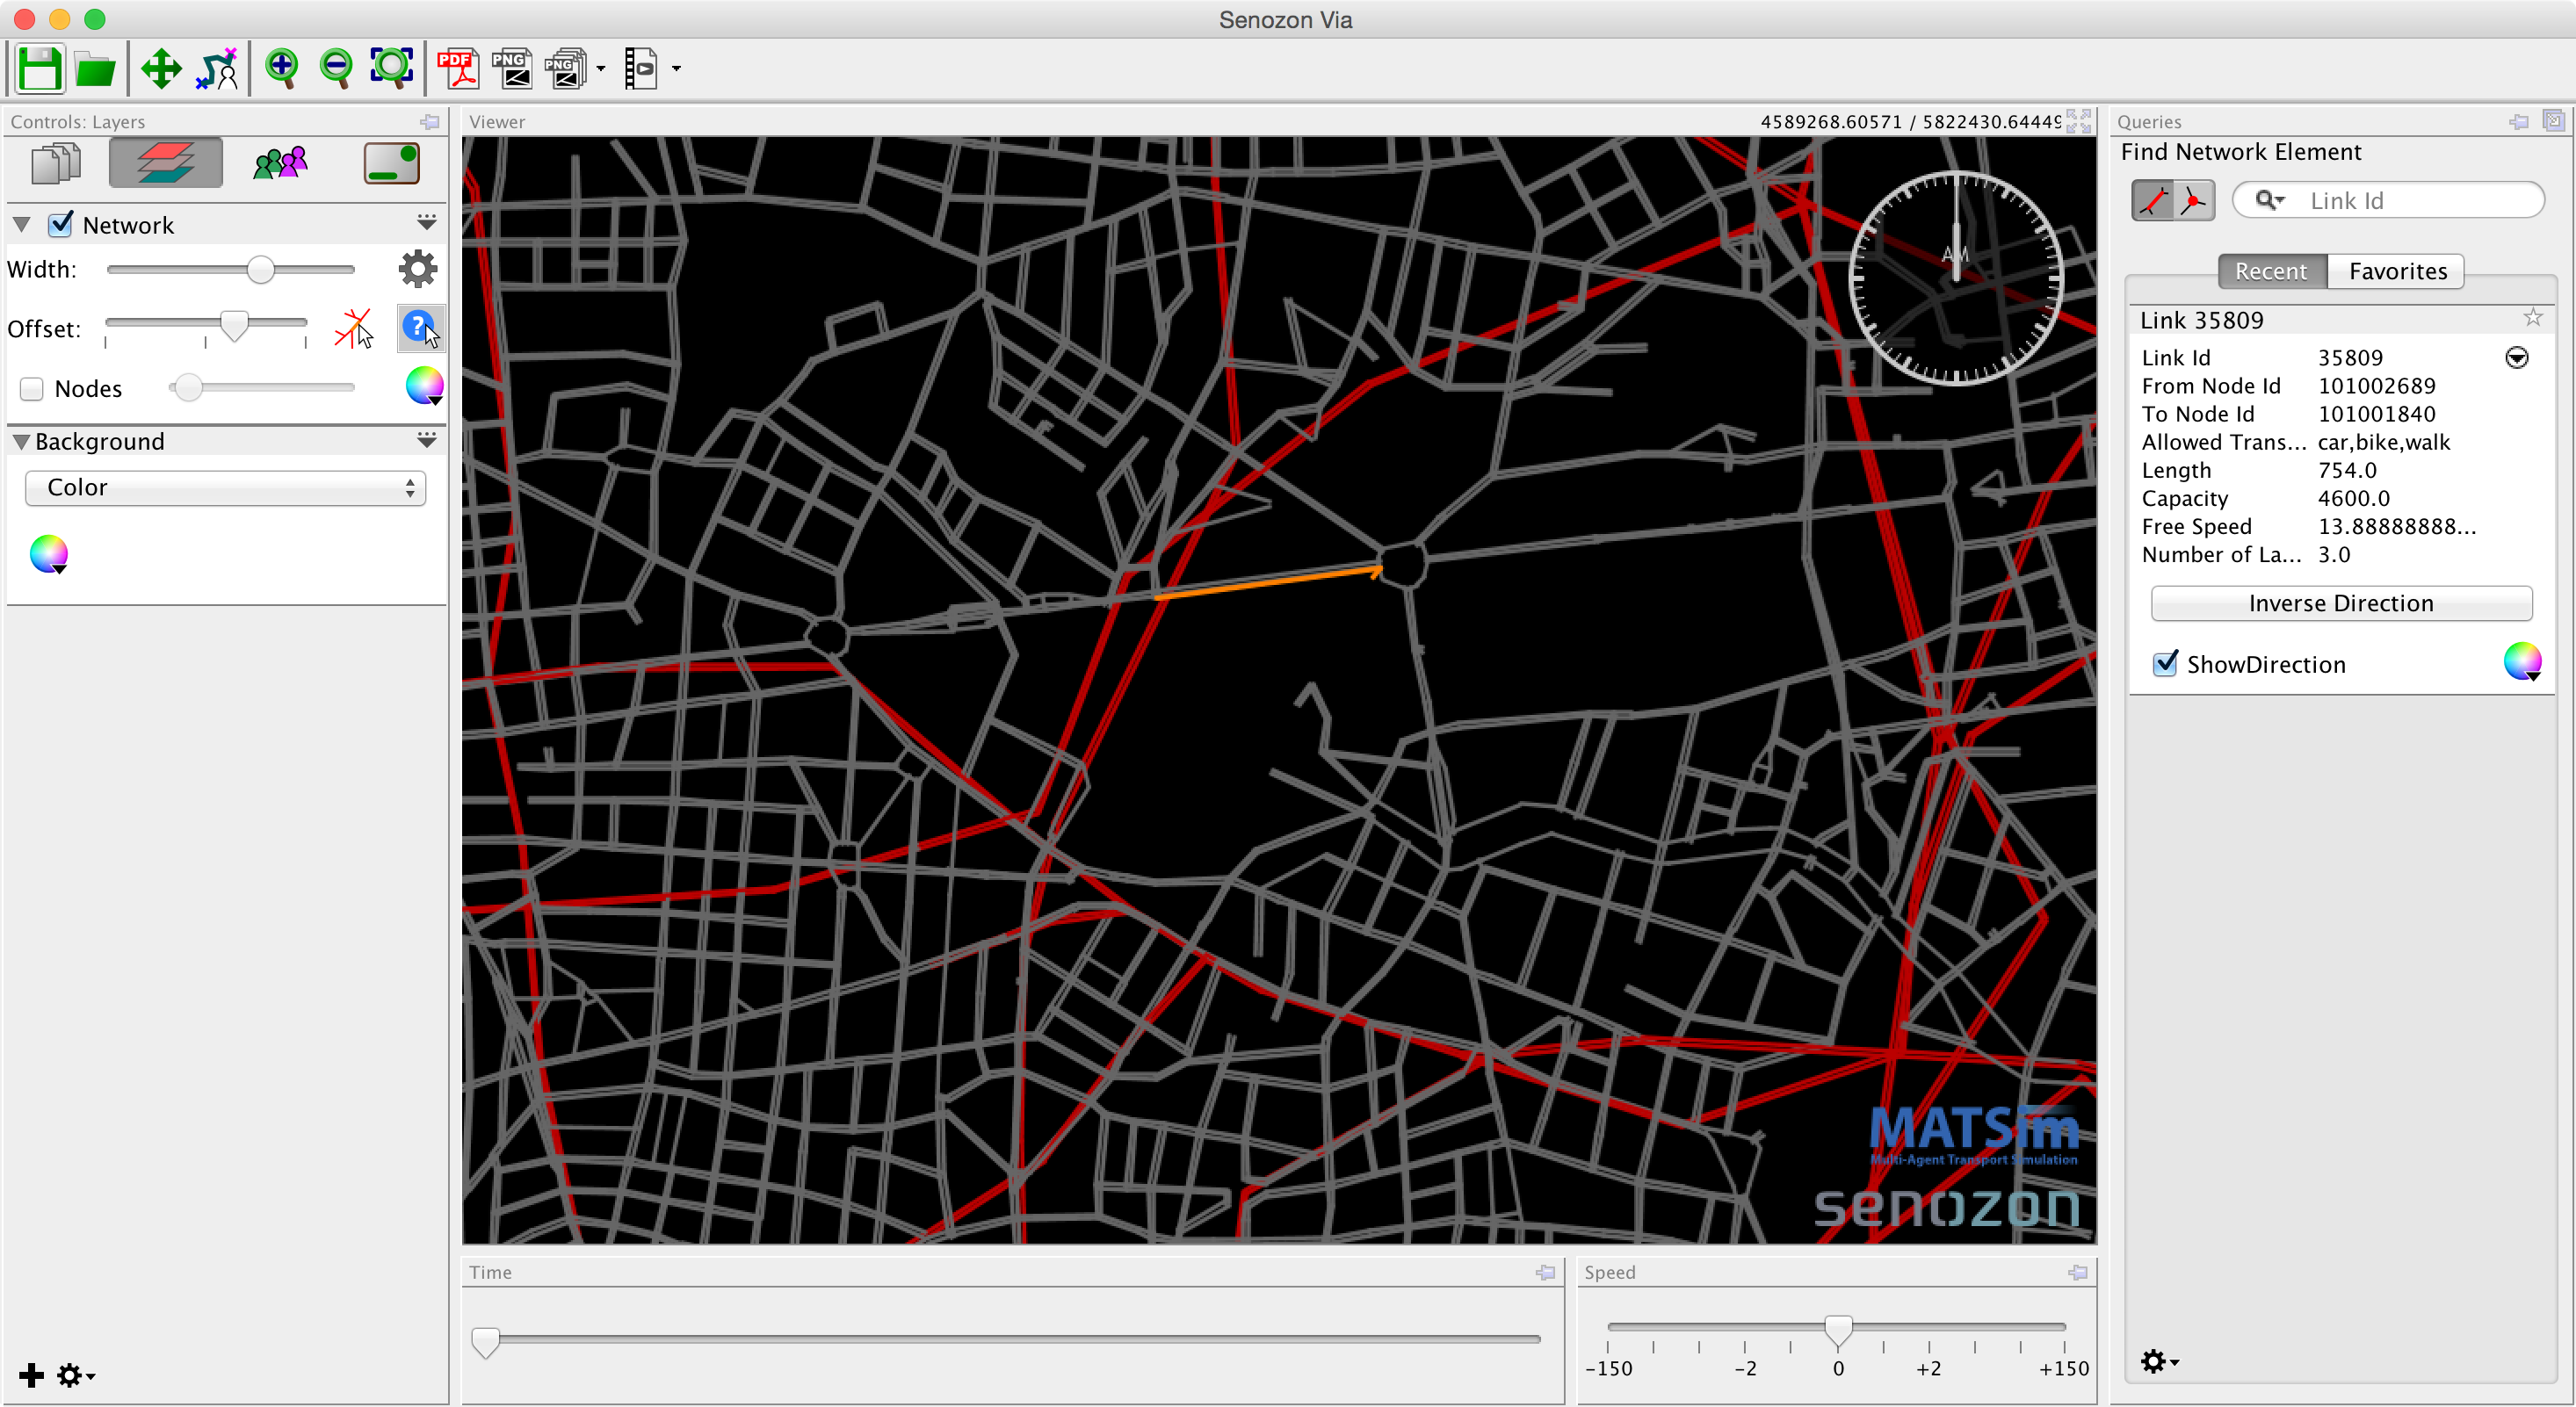
\includegraphics[width=1.\textwidth,angle=0]{./extending/figures/via/window.png}}%
{}

By default, \Via{}'s window looks similar to the one shown in Figure~\ref{fig:via:window}.
To add a file as a data source, the file can either be drag-and-dropped onto the layers
list left of the black visualization area, or by choosing \lstinline|Add Data...|
from the \lstinline|File| menu. To add a layer, the little plus icon in the lower left of
the window can be pressed, or by choosing \lstinline|Add Layer...| from the \lstinline|File|
menu. To get started, it's usually the best to add a network and (small) events
file from MATSim to Via, and create a \lstinline|Network| layer and a \lstinline|Vehicles| layer.

Elements shown in the visualization area like the network or vehicles can
be queried. Queries are usually provided by layers, made available with buttons
with question-mark icons. Clicking such an icon activates the corresponding
query mode, and any subsequent click on the visualization area will run the
query.
Query results are shown on the right side of the visualization area.
Figure~\ref{fig:via:window} shows a network query for links.
One query is a bit special and is globally available, and not linked to a
layer: querying an agent plan. This query is available from the toolbar, next to
the icon to shift the visualization view around.

Once a query has been made, \Via{} often allows to do another query based on the
current query results. By right-clicking in the visualization area, a popup menu
appears with more options regarding the last query, as well as additional
queries that are possible. Examples of such queries are: \lstinline|Select Link Analysis|
given a link, \lstinline|Select Facility Analysis| given a facility, \lstinline|List Transit Lines| that
use a given link, or \lstinline|List Passengers| if a transit vehicles was queried in the
first place.

% ##################################################################################################################
\section{Use Cases and Examples}
% ===================================================================================
\subsection{Agent Visualization}
The animated visualization of agents moving around in the modeled area was one
of the main features \Via{} was originally developed for. To do this, \Via{}
only needs the \lstinline|network.xml| and \lstinline|events.xml| files from a MATSim run
as data sources. For the visualization, a \lstinline|Network| layer, \lstinline|Vehicles| layer and
Activities layer must be created. With this setup, vehicles will move around in
the visualization area when the time progresses, and agents performing
activities will be represented as colorful dots.

The visualization can be further customized: With the addition of a \lstinline|population.xml| file, more detailed activity coordinates can be loaded to have a
better distribution of the activity locations (MATSim's events file does not
contain coordinates for activities, only the assigned link id. So by default,
all activities taking place on a link are first shown at the location of
the link's to-node). Also, vehicles and groups of vehicles can be styled
differently: It is possible to visualize transit vehicles with a square shape
with colors representing the occupancy of the vehicles, pedestrians or
cyclists in a multimodal simulation can be shown as circles, and private cars
can be displayed with a triangular shape with colors representing their
absolute speed or their speed relative to the allowed maximum speed on the link
they're on (see Figure~\ref{fig:via:vehicles}). As mentioned above, arbitrary
groups of vehicles can be styled differently, which is useful to highlight
special agents, e.g.,\,when simulating a fleet of electric vehicles, a car sharing
fleet, or agents simulated with special routing guidance.

It is possible to load arbitrary attributes for agents and use those attributes
as well for visualization purposes, e.g.,\,having different colors for vehicles
driven by agents that are employed, have a high income or are within a certain
age range.

\createfigure%
{Vehicles in Via}%
{Vehicles in Via: green triangular symbols represent private cars, pink rectangular symbols public transport vehicles }%
{\label{fig:via:vehicles}}%
{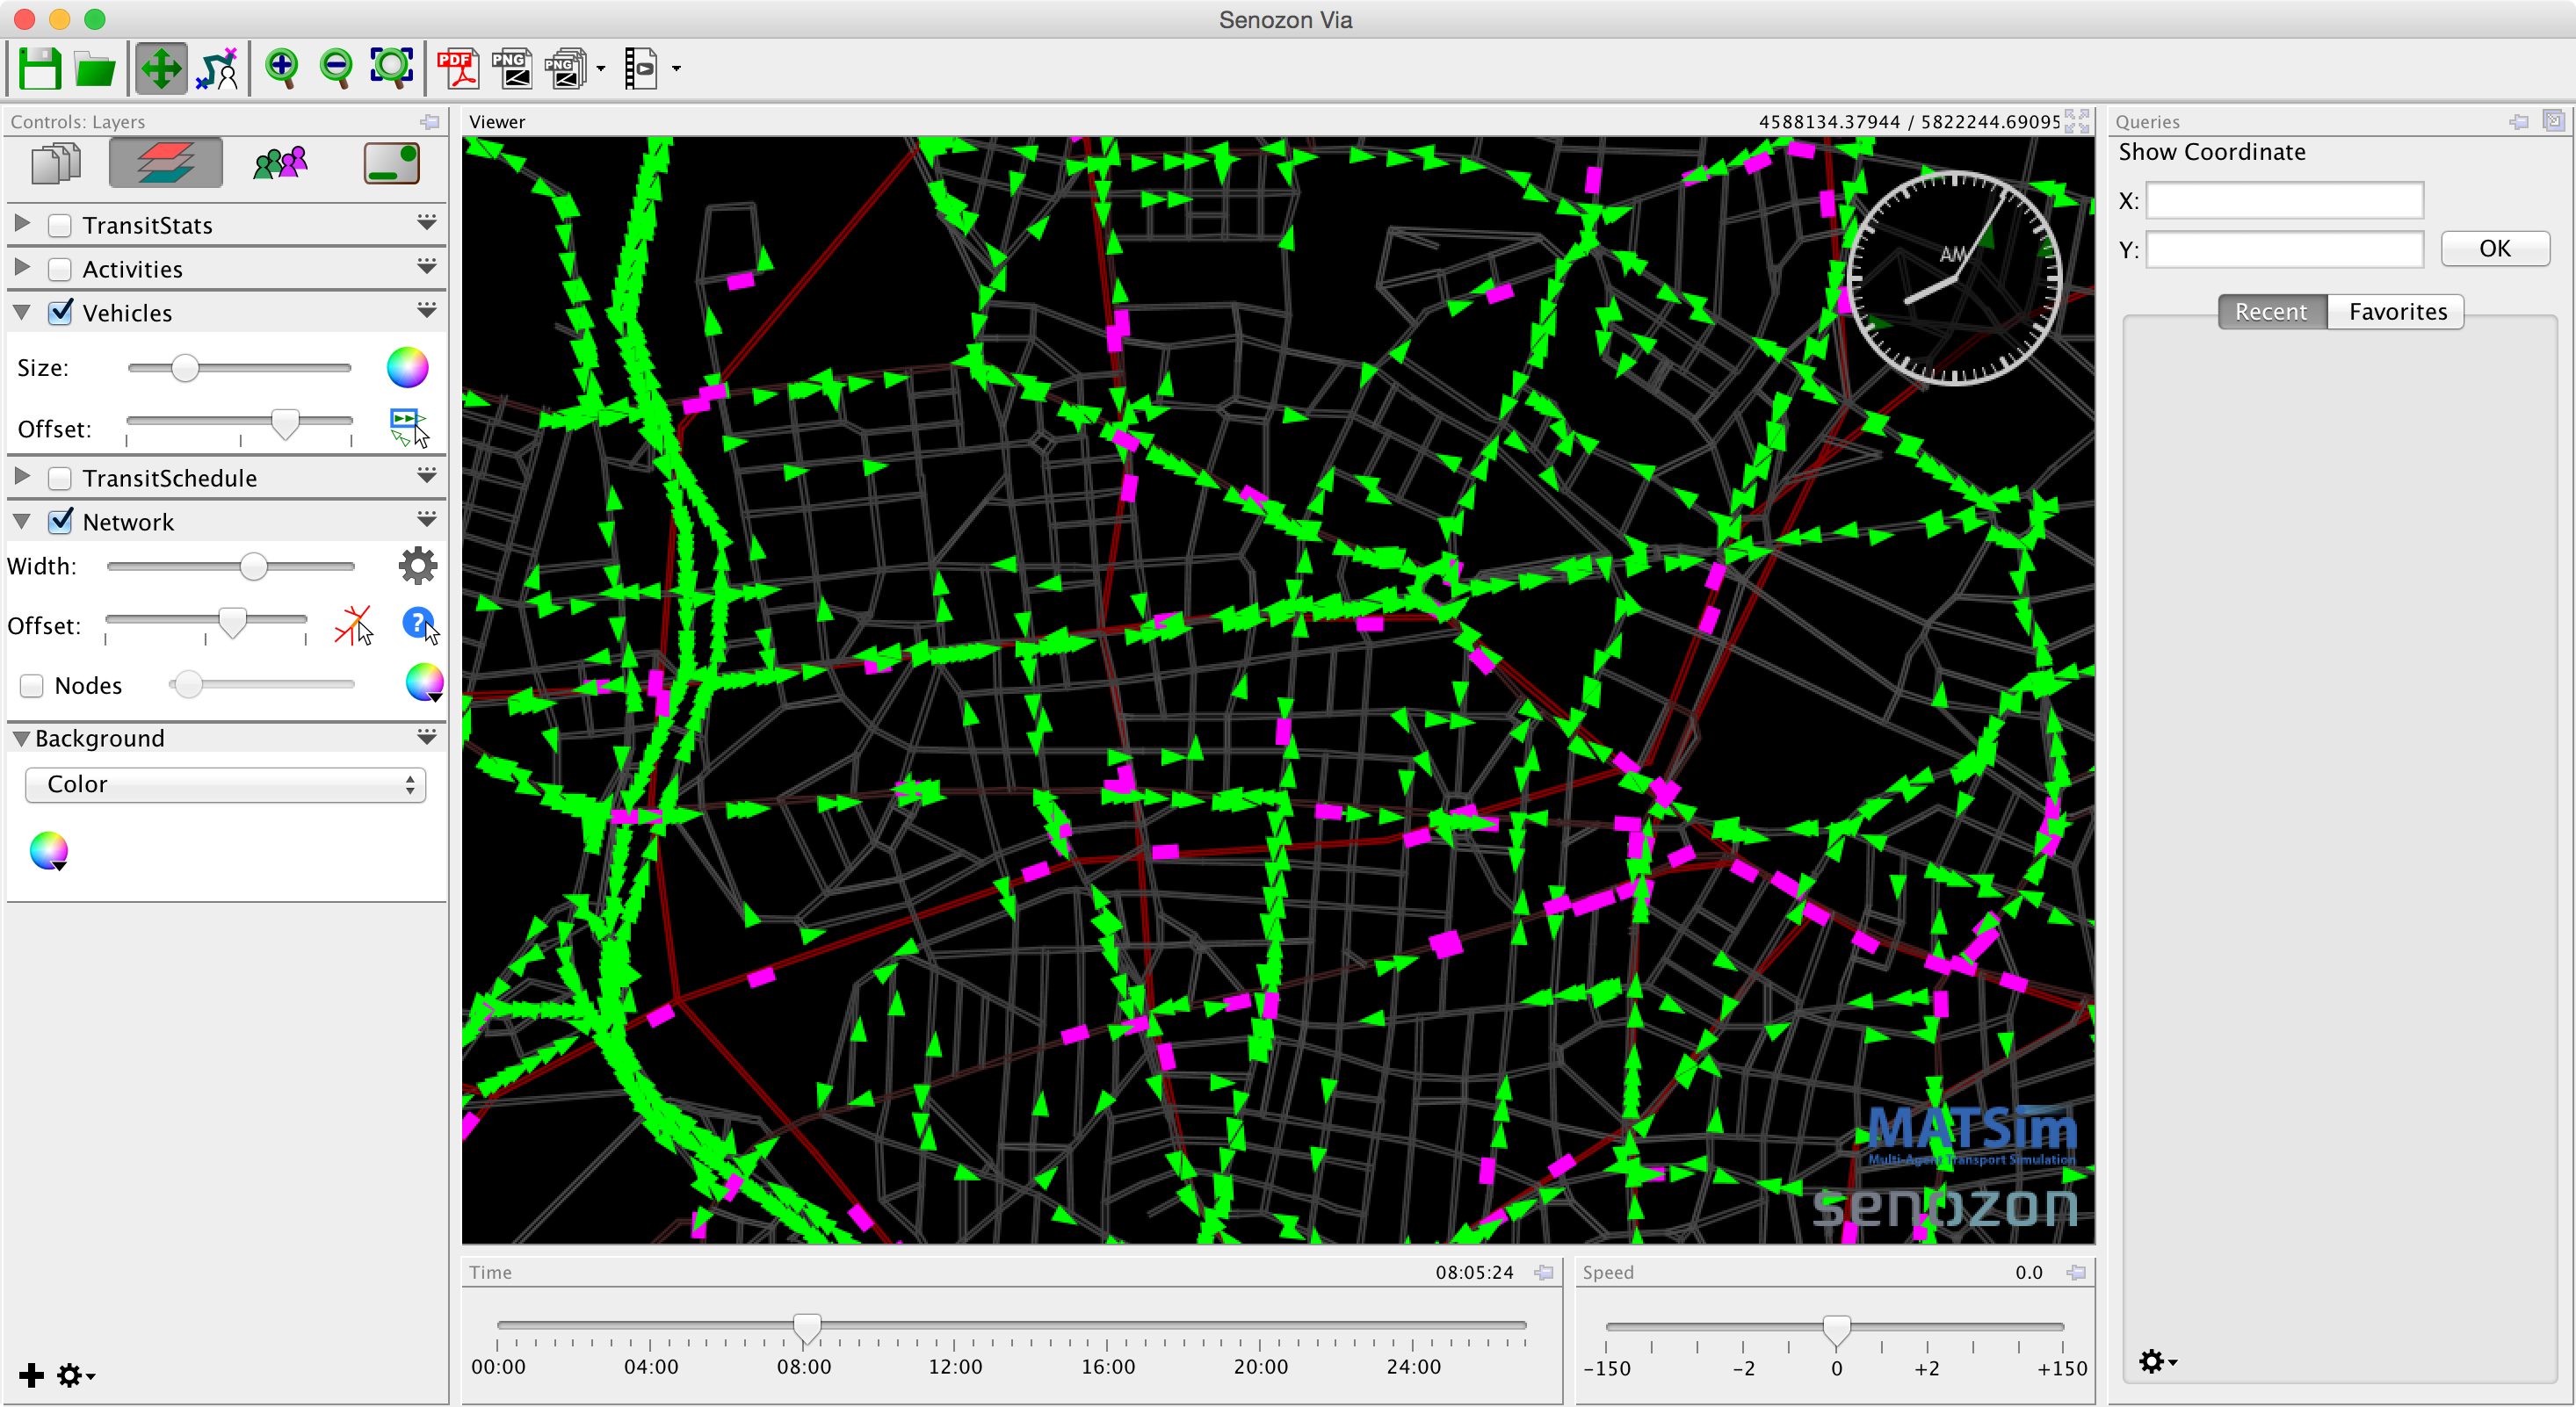
\includegraphics[width=1.\textwidth,angle=0]{./extending/figures/via/vehicles}}%
{}

% ===================================================================================
\subsection{Facility Analysis}
Activity facilities allow for very detailed modeling in MATSim, especially
considering the functionality provided by the destination innovation module
(Section~\ref{ch:destinationchoice}). \Via{} provides several unique ways to
analyze the mobility effects on and from facilities.

For each facility, a detailed analysis can be performed showing the number of
agents arriving at, departing at or staying at a facility over the simulated
time. The numbers can be differentiated by the type of activity the agents
perform at the facility, by the transport mode they arrive or depart with, or by
arbitrary other agent attributes that were loaded by users.

An alternative analysis is similar to the---for transport planners---well known
\lstinline|Select Link Analysis|, but for facilities: the \lstinline|Select Facility Analysis|. This
analysis shows the combined link loads produced by agents arriving or departing
at a facility, showing from which regions agents visit a specific facility and
what routes they use for this. Figure~\ref{fig:via:selectFacilityAnalysis} shows
such an example.

\createfigure%
{Select Facility Analysis}%
{Select Facility Analysis: Links used to travel to and from a facility are highlighted}%
{\label{fig:via:selectFacilityAnalysis}}%
{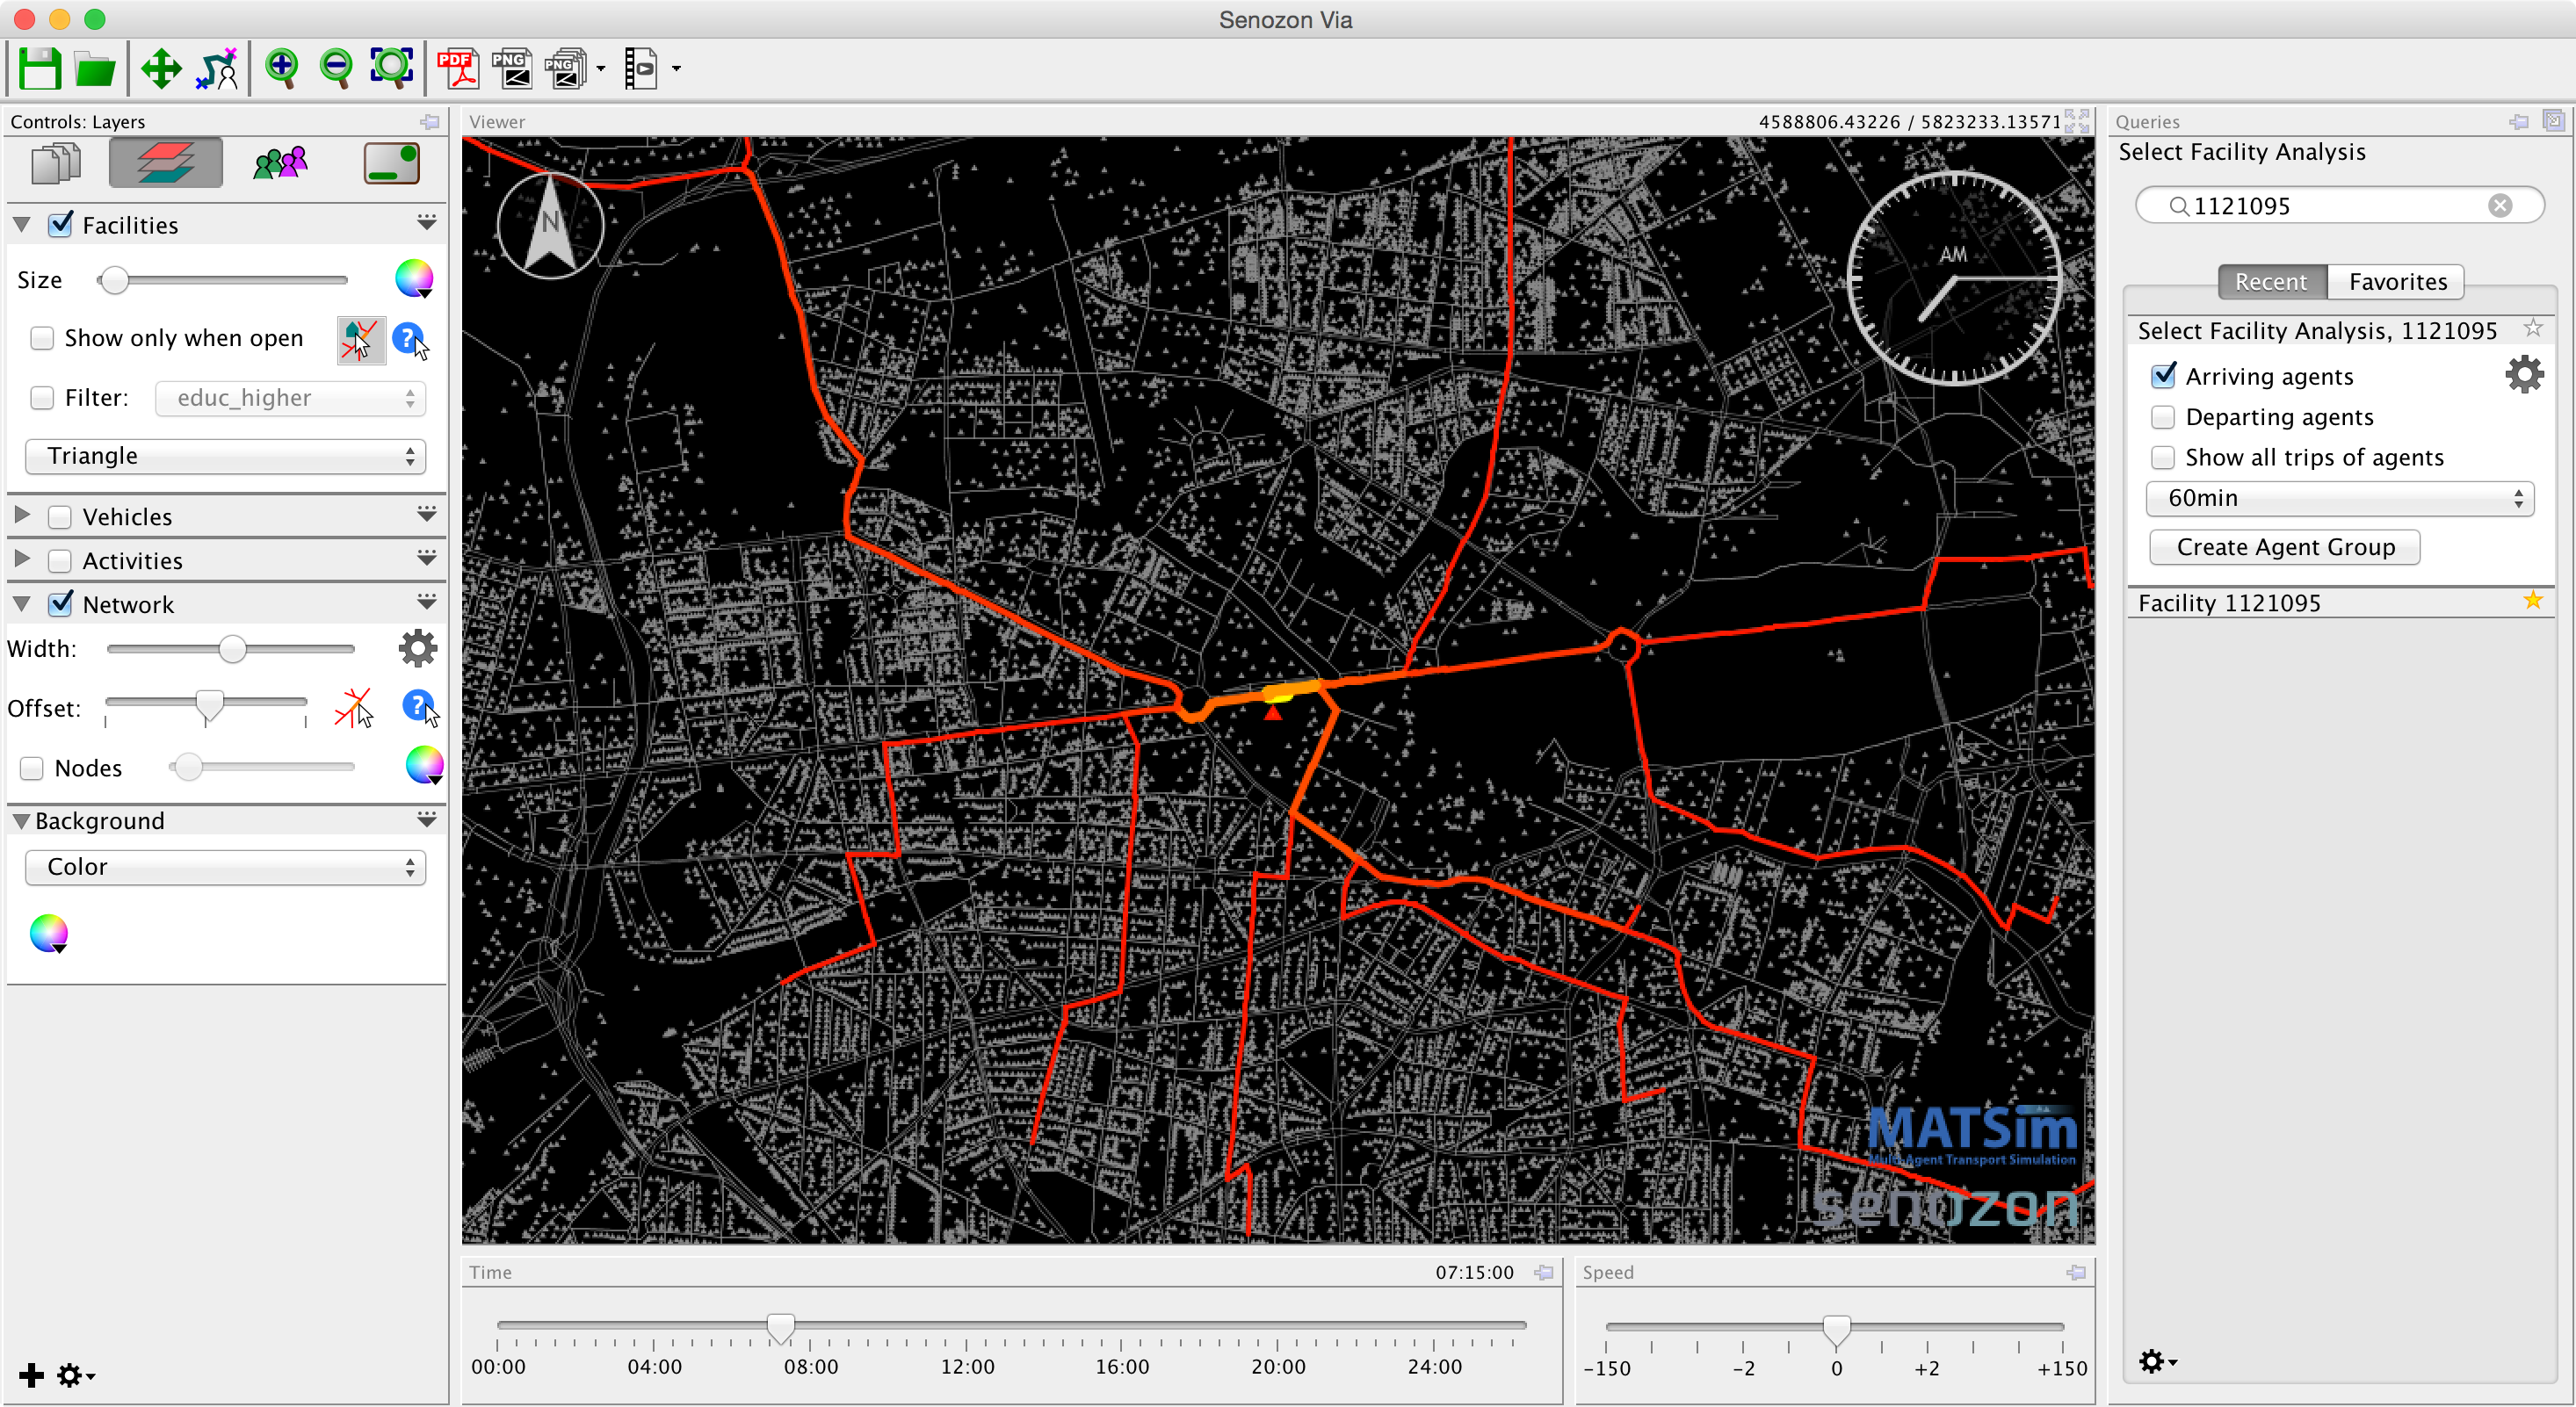
\includegraphics[width=1.\textwidth,angle=0]{./extending/figures/via/selectFacilityAnalysis}}%
{}

% ===================================================================================
\subsection{Public Transport Analysis}
The public transport plugin provides many different functionality for analyzing
public transport simulations. It starts with providing the specified vehicle
types as agent attributes, so the vehicles can be visualized differently based
on the vehicle type they represent. Also, the absolute or relative
occupancy of a transit vehicle is provided as attribute, agent allowing transit
vehicles to be visualized accordingly. For stop locations, the number of
passengers waiting for a bus or train can be plotted over the time of day, and
the occupancy along a bus or train route can be visualized.

A special, but very useful visualization is the "Route Flow" analysis. This
shows in a visually appealing way the number of passengers that travel between
two stops along a route---for all possible stop combinations.
Figure~\ref{fig:via:ptrouteflow} shows an example of such a route flow with the
route of the transit line shown in the background.
It can be easily seen that the demand on the bus route is more or less split in two: A
first travel demand up to about the first third of the route, and then it again
collects passengers that all want to go to one of the last stops along the
route. This could indicate that it might make sense to split the line in two.

\createfigure%
{Passenger flows on a transit line}%
{Passenger flows on a transit line}%
{\label{fig:via:ptrouteflow}}%
{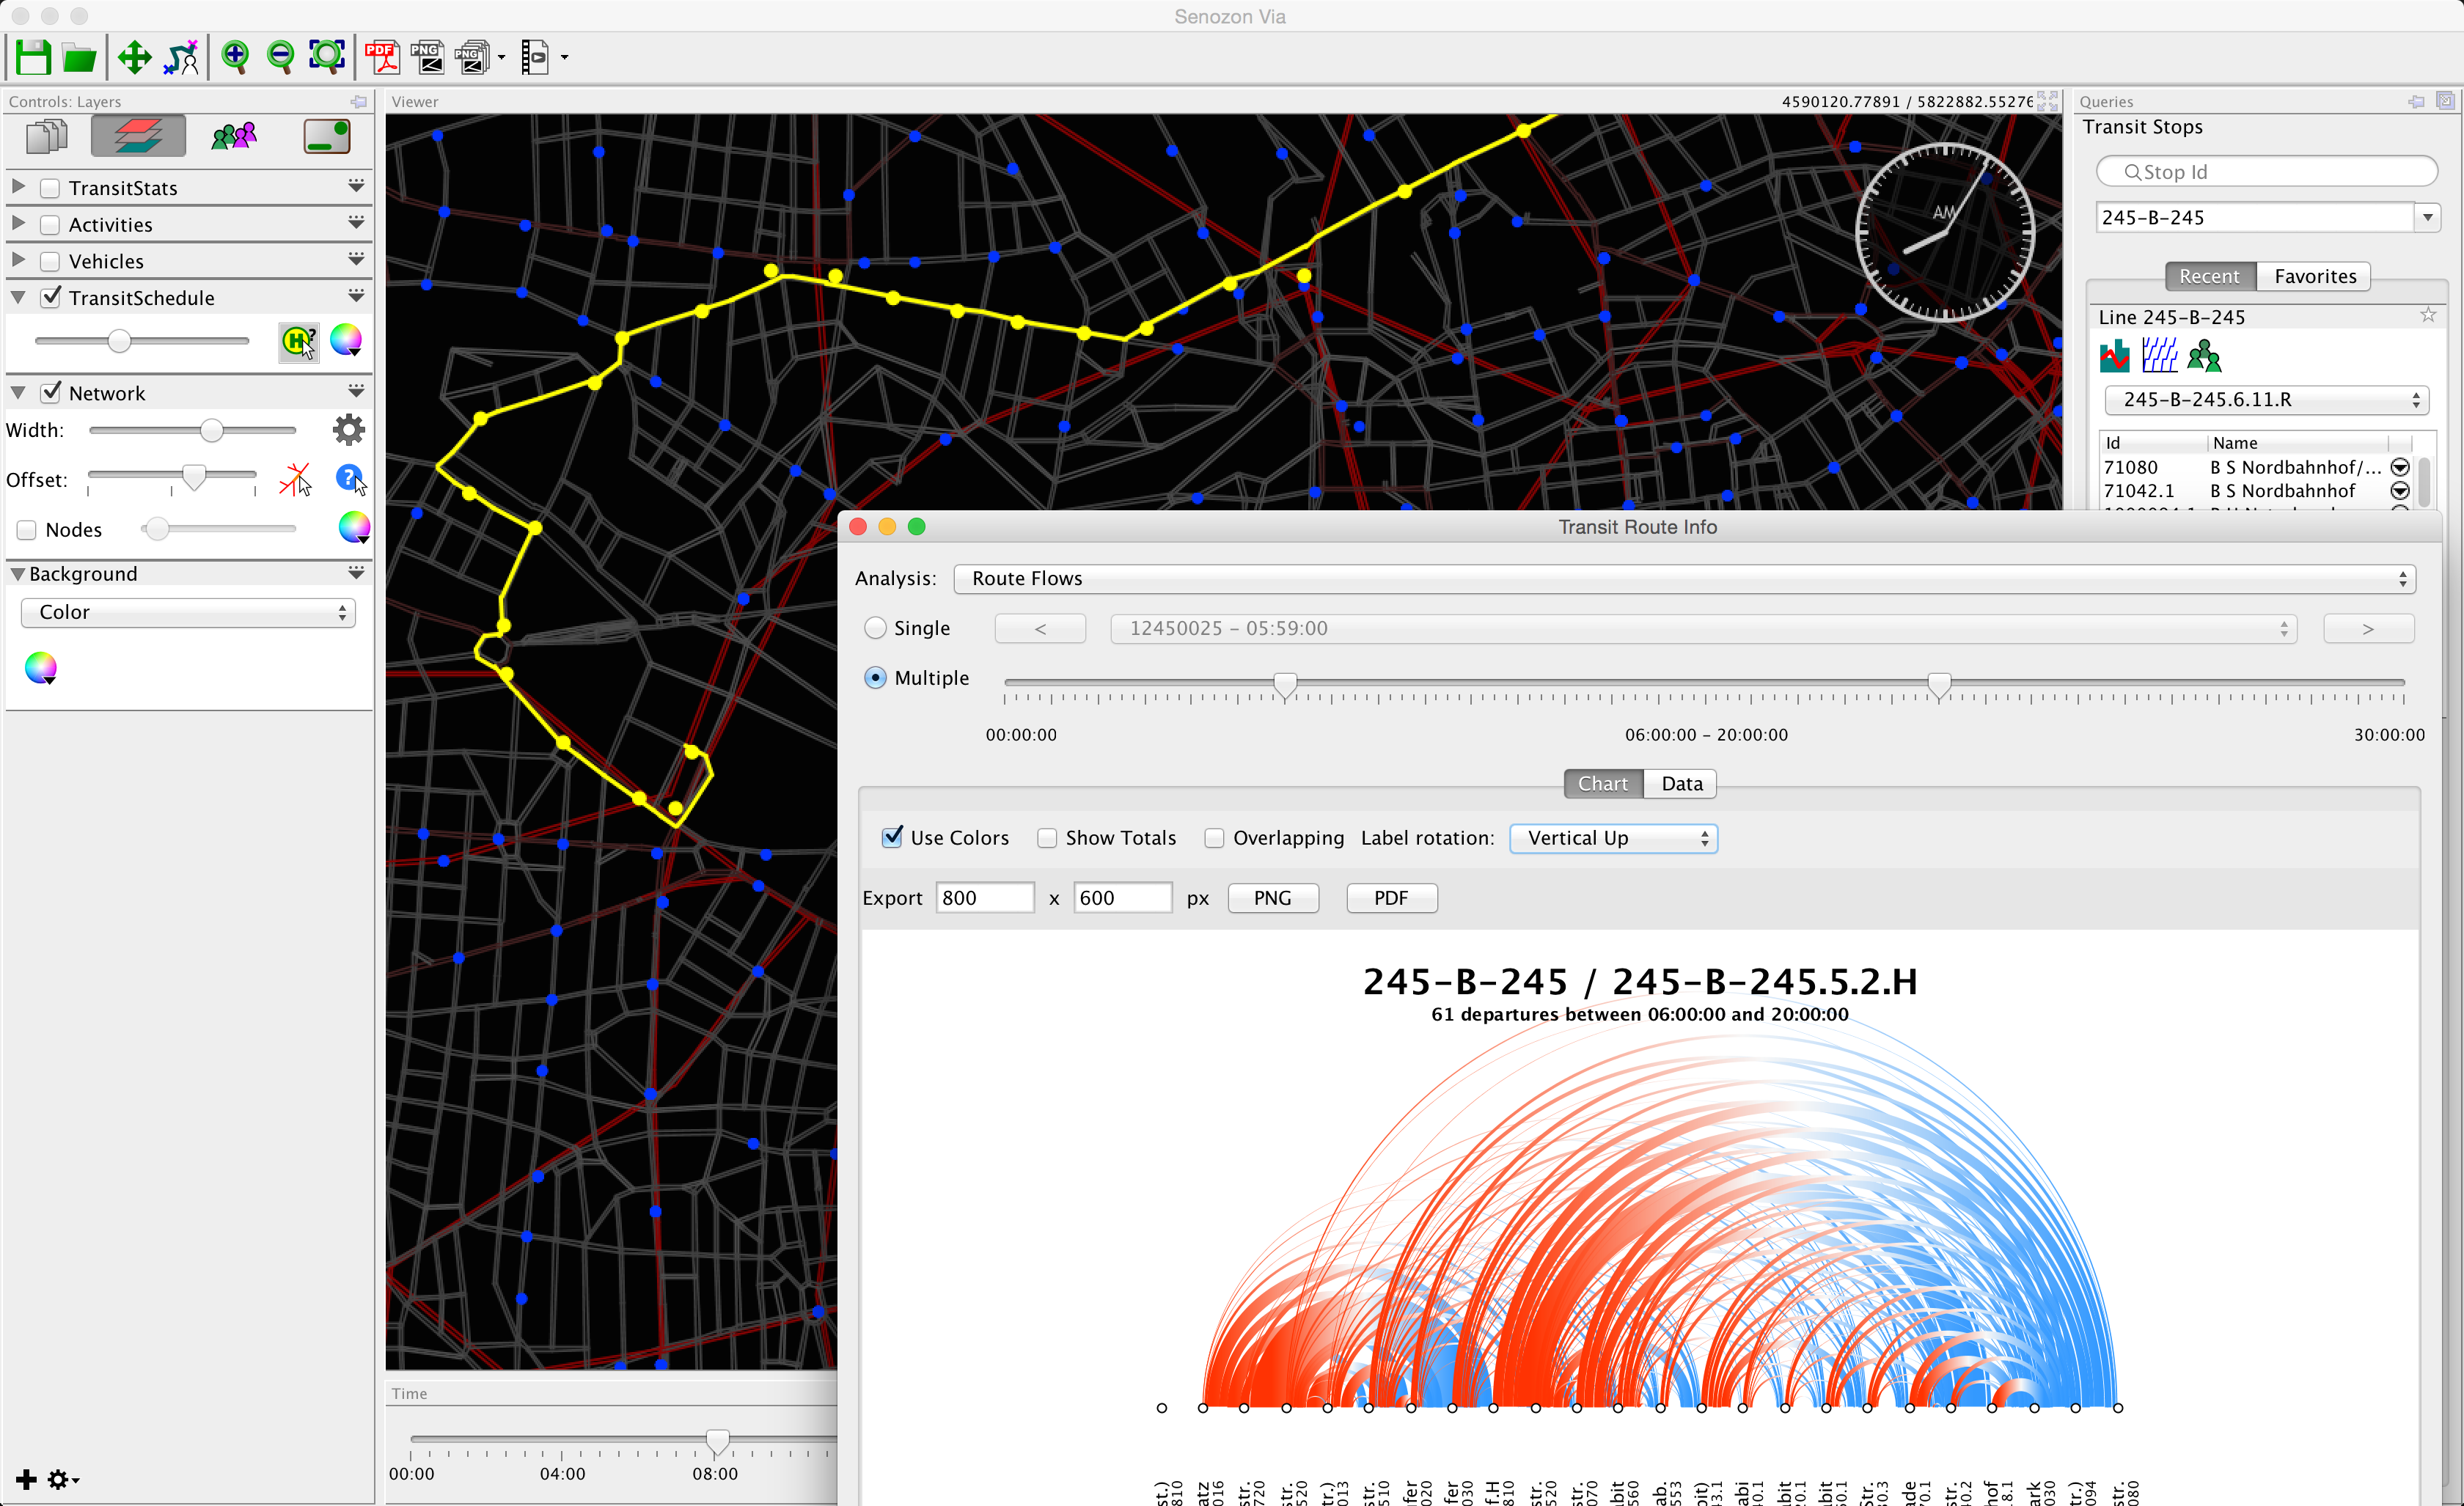
\includegraphics[width=1.\textwidth,angle=0]{./extending/figures/via/ptrouteflows}}%
{}

% ===================================================================================
\subsection{Scenario Comparisons}
A typical use case of MATSim is to simulate a base case and then one or more
case studies. Comparing scenarios then becomes an important step in the analysis
of the different case studies. \Via{} allows to compare the link volumes of two
scenarios visually by coloring the network with the absolute or relative
difference of the link volumes between two models. In the future, other
differences like average speeds will supported too. The differences are
time-dependent, aggregated over time bins of down to 15\,minutes.

% ===================================================================================
\subsection{Aggregating Data}
While MATSim requires and produces a lot of disaggregated data, it still often
is necessary to aggregate data to make statements or predictions about a
simulated scenario. \Via{} provides a powerful mechanism to easily build
arbitrary aggregations of available data. Such data can either be point data
(like activity locations, trip start locations, GPS points or any other spatial
point data) or origin-destination data (like trips with a start and end
location, or the relation of an activity location to the home location of the
agent performing the activity). While \Via{} provides activity locations, trip
start and trip end locations as well as facility locations automatically as point data
sources for aggregation, and the trips performed by agents as O-D data sources,
any tabular custom data with coordinate attributes can also be used for this. 

Data can be aggregated into a rectangular or hexagonal grid, where the cell-size
can be specified by the user, or into arbitrary zones provided as \lstinline|ESRI Shape| file by the user. The data points can be filtered by any of the
available attributes, and the aggregation can either just count the data points
in each region, or build the sum, the minimum or maximum or average of an
attribute of the data points.

With the activity locations provided by an
\lstinline|Activities Layer|, the following (and more) aggregations are possible:
\begin{compactitem}
  \item Show the number of performed activities per region
  \item Show the number of performed work activities per region
  \item Show the number of work activities starting after 10\,AM per region
  \item Show the average duration of work activities starting after 10\,AM per
  region
\end{compactitem}
Similarly, with the trips data provided by a \lstinline|Vehicles| layer, the following
exemplary aggregations are possible:
\begin{compactitem}
  \item Show the number of trip starts per region
  \item Show the number of trip starts with mode "car" per region
  \item Show the percentage share of trips starting with mode "car" in a
  region, compared to all trips starting in that region
  \item Show the average duration of trips starting with mode "pt" in a region
  after 11\,AM
\end{compactitem}

By the use of custom data tables, e.g.,\,containing more information about trips
like the from and to activity types they connect, the number of line switches if
it is a public transport trip (this requires the aggregation of MATSim's legs
to trips for analysis purposes), many more complex analyses are just a few
clicks away in \Via{}, like showing the average duration of car-trips starting
between 6\,AM and 8\,AM, going from "home" to "work".

\createfigure%
{Aggregation analysis}%
{Aggregation analysis: Number of performed activities during the whole day}%
{\label{fig:via:aggregation}}%
{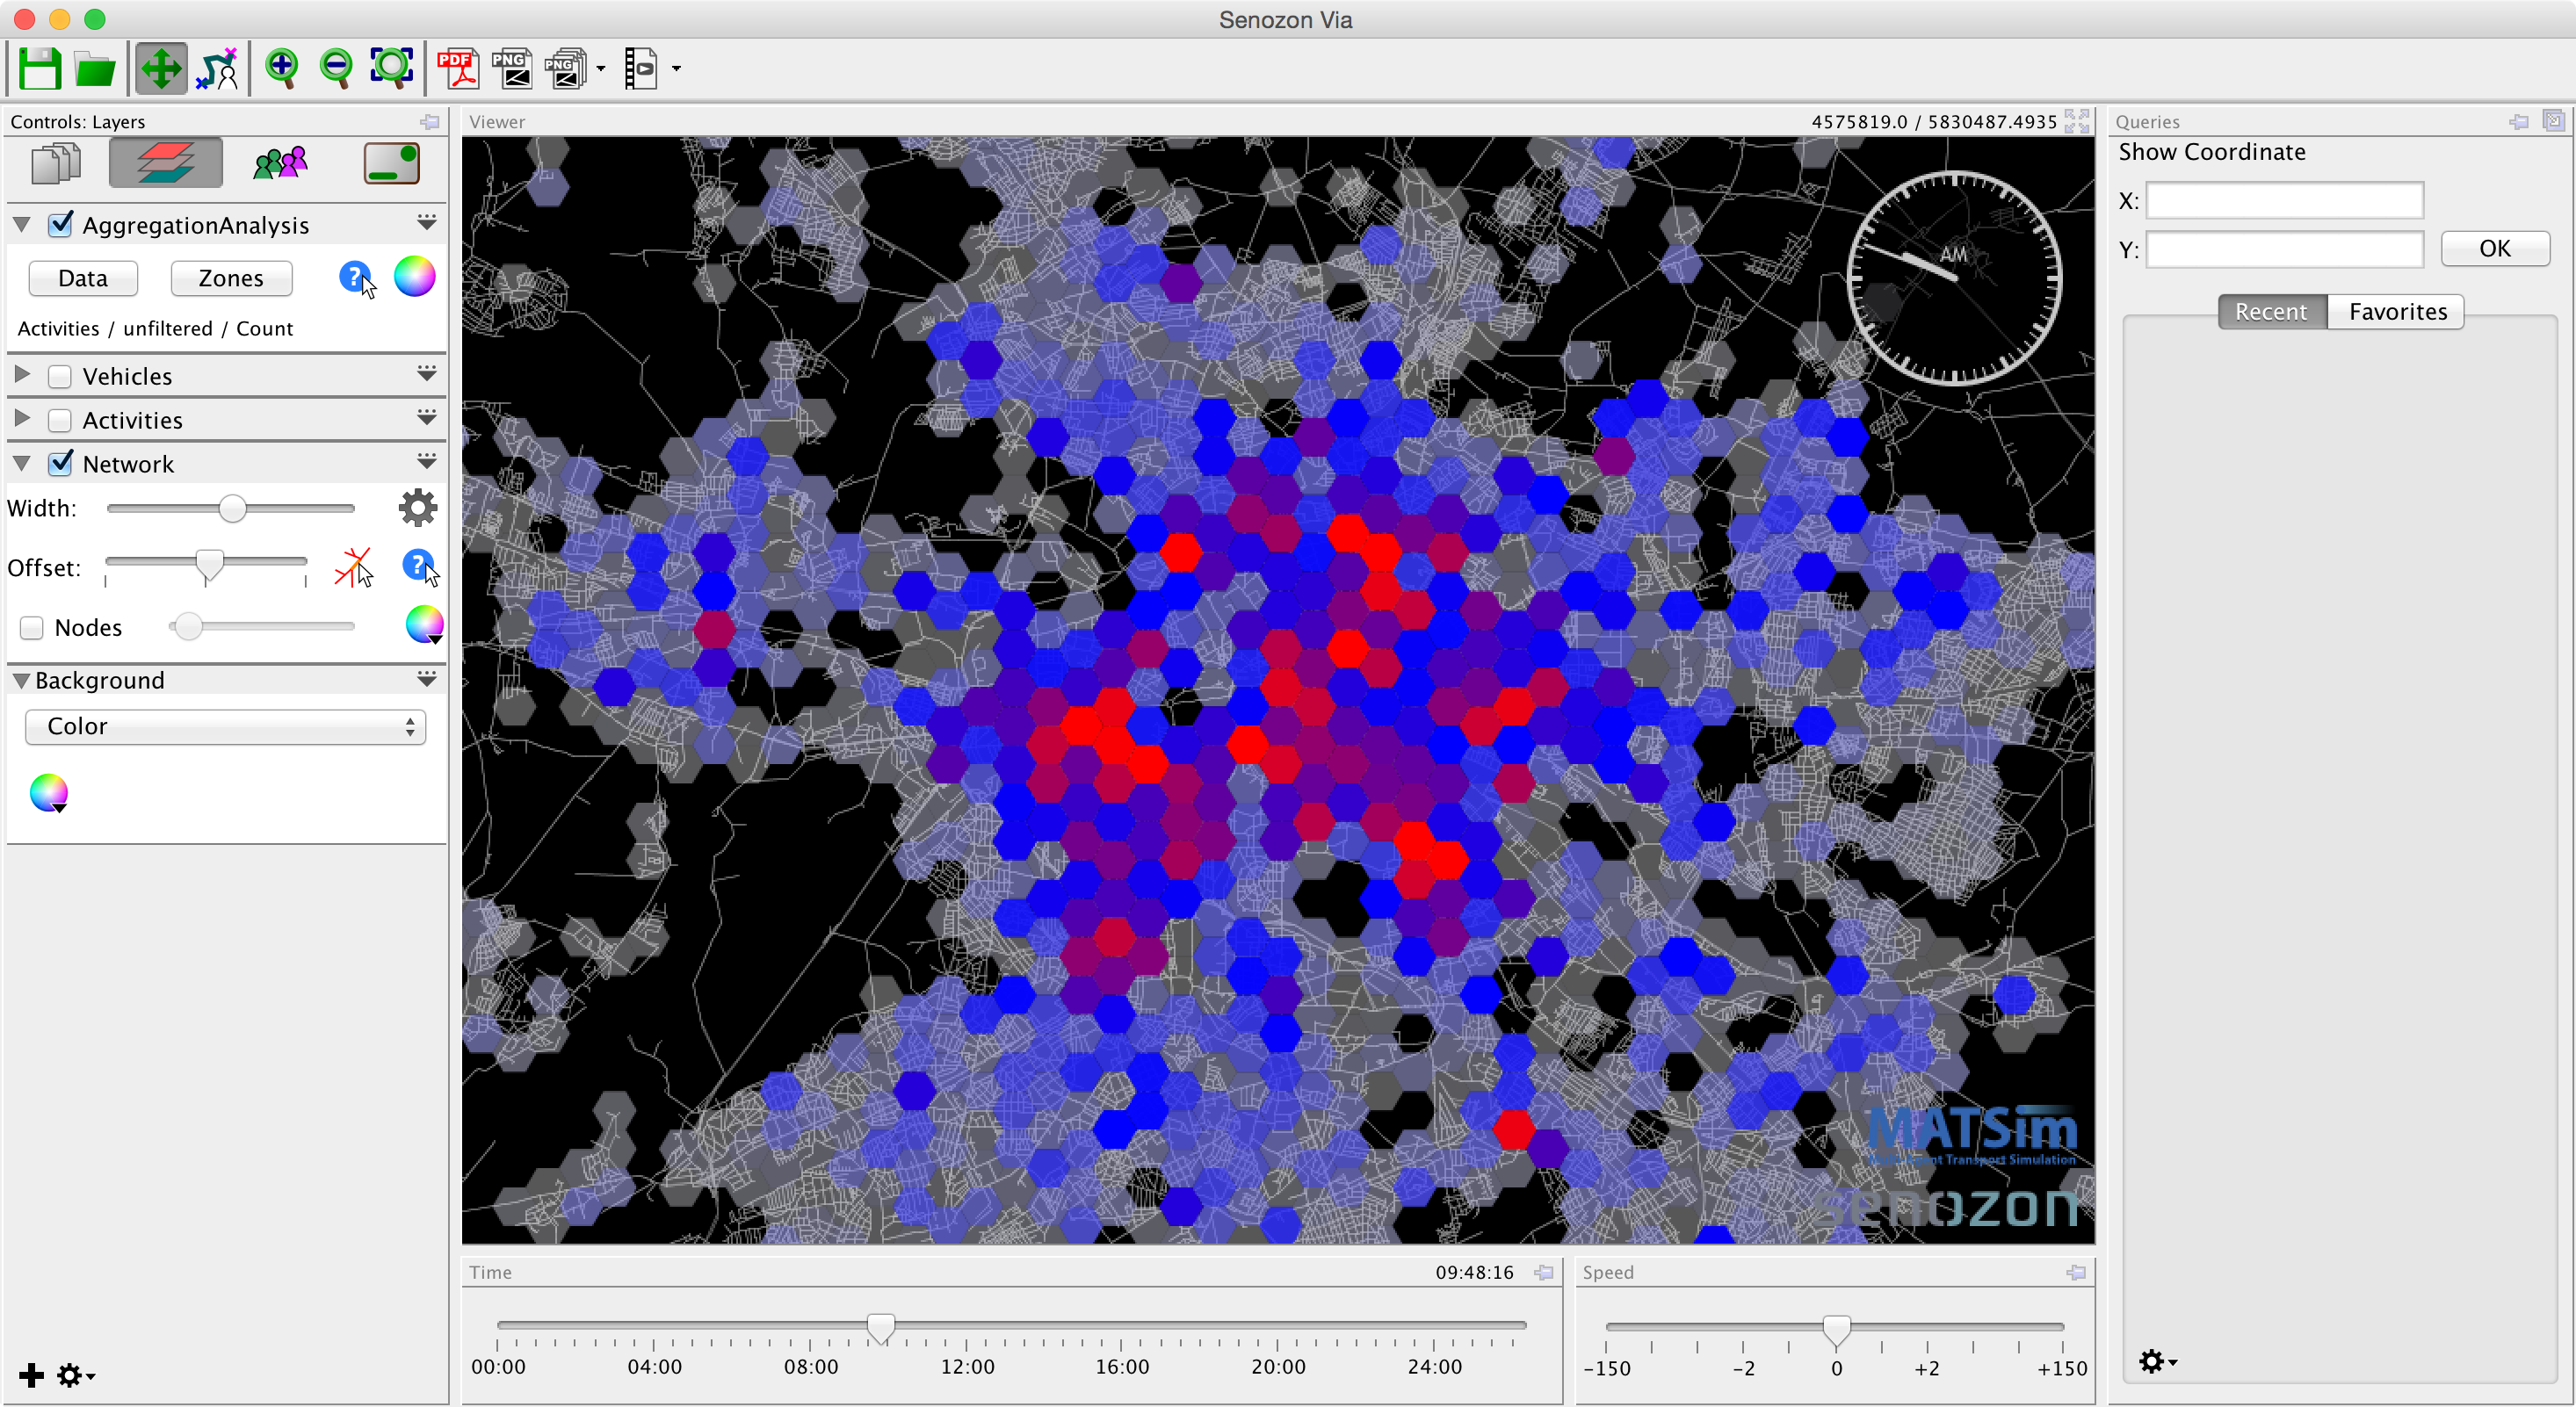
\includegraphics[width=1.\textwidth,angle=0]{./extending/figures/via/aggregation}}%
{}

% ################################################################################################################

